\documentclass[../report.tex]{subfiles}
\begin{document}	

\chapter{Design and simulation}
\gls{tpr} can be achieved in different ways, discussed in section \ref*{sec:active_pr}. In this thesis, the goal is to achieve \gls{tpr} using MEMS for a broadband spectrum including C and L bands. Moreover, the idea is to optimize the design to achieve high \gls{per} and low \gls{il}.  
	
	\section{Approach}
	\gls{tpr} with MEMS can be approached in 2 ways. In the first approach, initially a passive \gls{pr} can be designed by introducing asymmetry and another MEMS tunable waveguide is introduced which impedes polarization rotation by reintroducing symmetry in the effective waveguide. In the second approach, the technique is reversed i.e. the MEMS tunable waveguide is used to introduce asymmetry in the effective waveguide structure which rotates polarization. Without the MEMS structure the polarization is not rotated. In the design principle of the \gls{tpr} described here, the first approach is being followed.  
	
	\section{Designing the experiment}
	To design the geometry of the waveguide standard mode solver softwares are used. Both, Comsol\cite{comsol_2015} and CST \cite{cst_2015} are used to solve the modes in equation \ref{eq:helmholtz_eq_wg_general}. Mostly, in this thesis Comsol is used to find and optimize the port modes in 2-D geometry. Whereas, CST is used to optimize the 3-D structure by studying the transmission parameters (S-parameters) obtained for output port mode after running the simulation. Air cladding is considered around the Silicon base waveguide for setting up the simulation.
		
		\subsection{Design principle}
To design a \gls{pr} in nanometer scale, precision is a key factor. Index profile of chosen silicon can also affect the structural dimensions of the design in a rigorous manner. Meshing of the geometry, cladding dimensions and its material composition, frequency domain of the solvers etc. are the key things to watch for in designing the simulation in the mode solver softwares. As the idea is to make the \gls{tpr} as broadband as possible, it is necessary to do frequency analysis simulation for a wide-band spectrum in which the optical fibers for telecommunications work. As, the operating wavelength of the telecommunications optical fiber network in C-band and L-band are between $\SI{1530}{\nano\metre}$ and $\SI{1625}{\nano\metre}$, the corresponding frequency domain becomes $\SI{184.48}{\THz}$ - $\SI{195.94}{\THz}$.
	
		\subsection{Design A: Single stair Si waveguide on SOI with air cladding based on mode hybridization}
Initially, a single stair waveguide is being designed for \gls{pr}. To find out the dimensions for obtaining $45{^\circ}$ hybridized modes, Comsol 2D mode solver is used. 

\subsubsection{Optimized dimensions of bus waveguide}
At $45{^\circ}$, the components of the E-fields in the hybridized modes must be such that, $E_X \approx E_Y$. Hence, $\dfrac {E_{X_{mode}}} {E_{Y_{mode}}} \rightarrow 1$. As a result, 

\begin{equation}\label{eq:wg_dim_eq}
\sum _{mode}Real\left| \log _{10}\dfrac {E_{X_{mode}}} {E_{Y_{mode}}}\right| \rightarrow 0. 
\end{equation}

\begin{figure}[H] %h
	\centering
	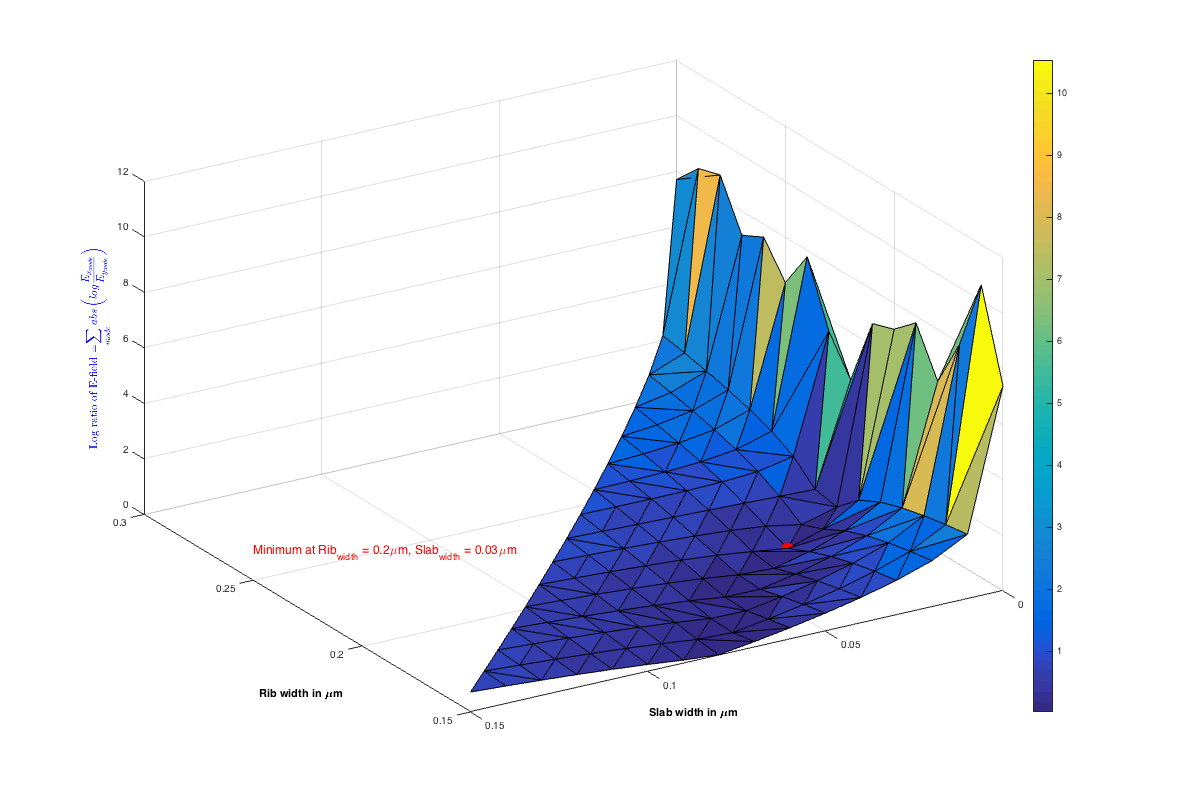
\includegraphics[width=1\textwidth]{3-graph-mode-sum}
	\caption{Summation of real part of absolute value of the logarithmic ratio of $E_x$ and $E_y$ fields plotted against rib and base width in an area chart using MATLAB}
	\label{fig:3_graph_mode_sum}
\end{figure}  
\noindent Hence, the minimum point on the graph represents the best dimensions on the waveguide for obtaining the hybridized modes at $45{^\circ}$. In this case the best dimensions were obtained at $Slab_{width}$ = 230nm and $Rib_{width}$ = 200nm. The total height of the waveguide is 220nm and the$Slab_{height}$ = 110nm. It can visualized that in the modes in Fig. \ref{fig:3_mode1_200_230} and Fig. \ref{fig:3_mode2_200_230}, that the effective modes are hybridized at $45{^\circ}$ for the first 2 fundamental modes obtained using Comsol simulation.
\begin{figure}[H] %h
	\begin{subfigure}[t]{0.45\textwidth}
		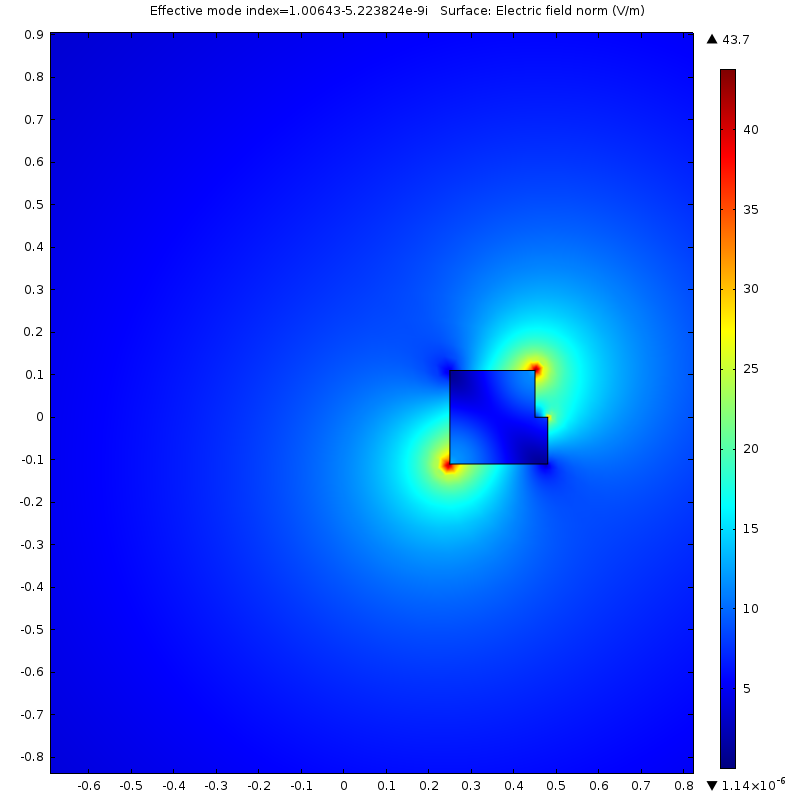
\includegraphics[width=\textwidth]{3-mode1-200-230}
		\caption{$1^{st}$ hybrid mode in the cross-section}
		\label{fig:3_mode1_200_230}
	\end{subfigure}
	\hfill
	\begin{subfigure}[t]{0.45\textwidth}
		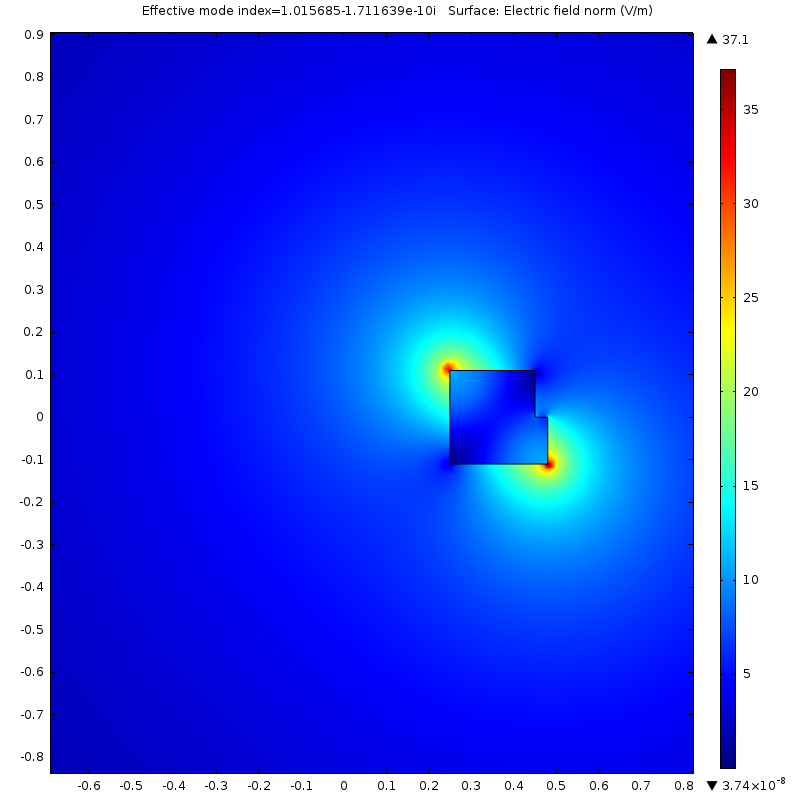
\includegraphics[width=\textwidth]{3-mode2-200-230}
		\caption{$2^{nd}$ hybrid mode in the cross-section}
		\label{fig:3_mode2_200_230}
	\end{subfigure}
	\caption{Hybrid modes in the cross-section with $Rib_{width}$ = 200nm, $Rib_{height}$ = 110nm, $Slab_{width}$ = 230nm, $Slab_{height}$ = 110nm, obtained using Comsol 2-D simulation}
\end{figure}

\begin{figure}[H] %h
	\begin{subfigure}[t]{0.45\textwidth}
		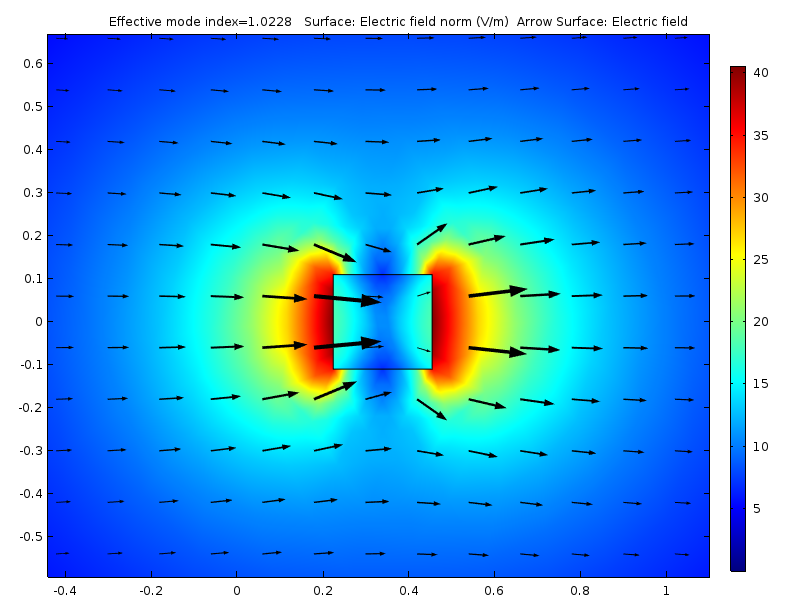
\includegraphics[width=\textwidth]{3-mode1-230-230}
		\caption{\gls{te} mode in the cross-section}
		\label{fig:3_mode1_230_230}
	\end{subfigure}
	\hfill
	\begin{subfigure}[t]{0.45\textwidth}
		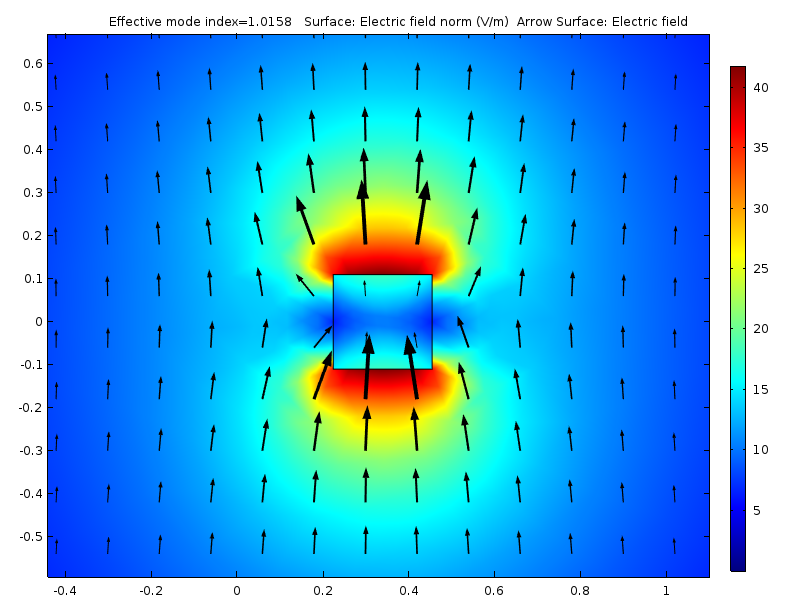
\includegraphics[width=\textwidth]{3-mode2-230-230}
		\caption{\gls{tm} mode in the cross-section}
		\label{fig:3_mode2_230_230}
	\end{subfigure}
	\caption{Hybrid modes in the cross-section with Width = 230nm, Height = 220nm, obtained using Comsol 2-D simulation}
\end{figure}

\noindent Also, since the port dimensions are different from the cross-section dimensions it is necessary to check if the 2 fundamental modes can be supported by the ports. Hence, port mode simulation for the first two fundamental modes in waveguide with dimensions 230$\times$220 nm is being run and the results obtained are displayed in Fig. \ref{fig:3_mode1_230_230} and Fig. \ref{fig:3_mode2_230_230}. This corroborates that the 2 fundamental modes \gls{te} and \gls{tm} are supported in the ports.\\

\noindent Next, the effective \gls{ri} for both the port modes are obtained using CST by doing a parametric sweep over the operating frequencies of C and L-band. The results are displayed in Fig. \ref{fig:3_effective_ri_200_230}. 

\begin{figure}[H] %h
	\centering
	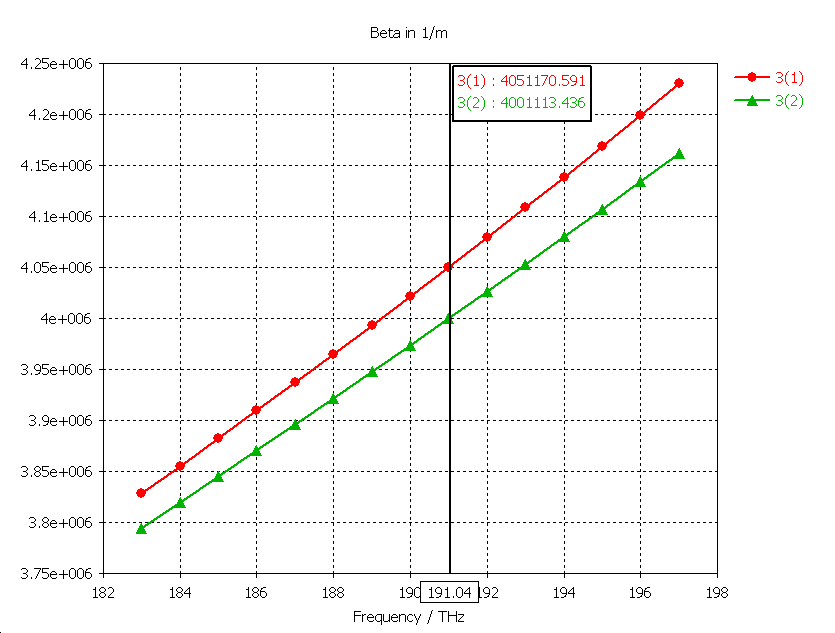
\includegraphics[width=0.9\textwidth]{3-effective-ri-200-230}
	\caption{Simulated effective \gls{ri} profile for the port modes in the cross-section of $Rib_{width}$ = 200nm, $Rib_{height}$ = 110nm, $Slab_{width}$ = 230nm, $Slab_{height}$ = 110nm, obtained using CST 3-D simulation}
	\label{fig:3_effective_ri_200_230}
\end{figure}

\noindent The required length of the cross-section is obtained using \ref{eq:jones_matrix_wp1}. Since, $\beta_1$ = $4.051 \times 10^6$  and $\beta_2$ = $4.001 \times 10^6$. Hence, $L = \dfrac{\pi}{\beta_1 - \beta_2} \approx 51nm$. This means the length of the stair cross-section would be around 51nm. Effective \gls{ri} is dependent on frequency and so the cross-section length is also dependent on the frequency. The length is calculated at around $\SI{191}{\THz}$, so that the whole of the band ($\SI{184.48}{\THz}$ - $\SI{195.94}{\THz}$) can be covered for a relative good performance. 

\begin{figure}[H] %h
	\centering
	\includegraphics[width=0.9\textwidth]{3-wg-design-1}
	\caption{Design of single-stair waveguide with initial dimensions at the port as width = 230nm and height = 220 nm. Stair cross-section dimensions are: $Rib_{width}$ = 200nm, $Rib_{height}$ = 110nm, $Slab_{width}$ = 230nm, $Slab_{height}$ = 110nm, and cross-section length = \SI{51}{\micro\meter}. The output port is along the Z-axis}
	\label{fig:3_wg_design_1}
\end{figure}

\noindent The 3D-design is simulated in CST with air cladding and with the dimensions calculated. The input and output ports are defined on the waveguide, which supports the two fundamental modes. As shown in Fig. \ref{fig:3_wg_design_1}, the stair cross-section can be envisaged if a Z-plane is cut in the asymmetric part of the waveguide.\\

\noindent Next, the S-parameters of the design are verified. The S-parameter is being labelled as follows,
\begin{equation}\label{eq:s_parameter_label}
SA(M),SB(N),
\end{equation}
where A=output port, B=input port and M,N = mode number. For example, S2(2),S(1)1 means that input port is 1 and the mode is 1 whereas, output port is 2 and the mode at the output port is 2. Hence, S2(1),S1(2) and S2(2),S1(1) needs to be checked along with S2(1),S1(1) and S2(2),S1(2) for calculating the \gls{per}. The S-parameters obtained from the simulation shown in Fig. \ref{fig:3_stair_s_param_200_230} (for, 200nm$\times$230nm) verifies that the model works according to the design principle with good \gls{per} over the whole band. 

%For example, the $PER_{191 THz} = 10 log_{10} $

\begin{figure}[H] %h
	\centering
	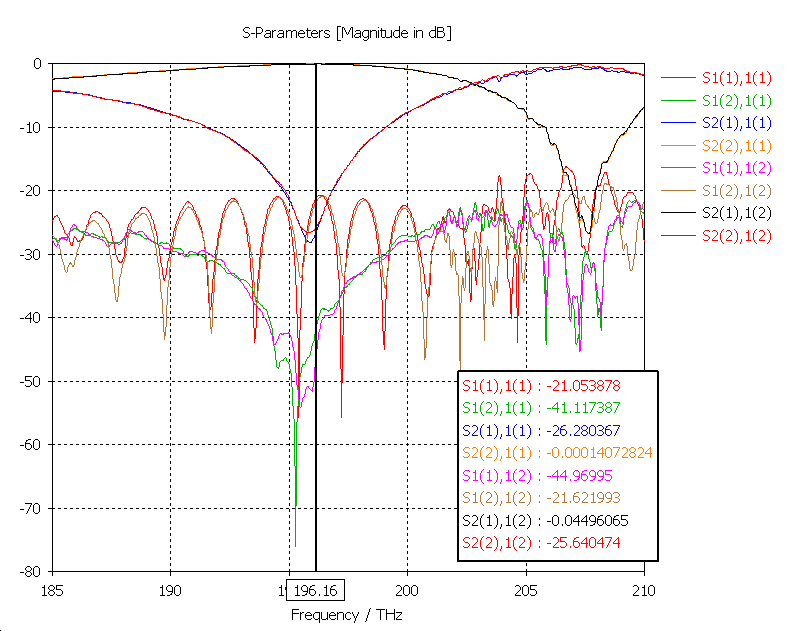
\includegraphics[width=0.9\textwidth]{3-stair-s-param-200-230}
	\caption{Simulated S-parameters in the single-stair waveguide with initial dimensions at the port as width = 230nm and height = 220 nm. Stair cross-section dimensions are: $Rib_{width}$ = 200nm, $Rib_{height}$ = 110nm, $Slab_{width}$ = 230nm, $Slab_{height}$ = 110nm, and cross-section length = \SI{51}{\micro\meter} obtained using CST 3-D simulation}
	\label{fig:3_stair_s_param_200_230}
\end{figure}

\subsubsection{Optimized dimensions of MEMS waveguide}
After finding the dimensions of the passive \gls{pr}, the design of the \gls{mems} tunable waveguide was designed to neglect the effect of rotation. Intuitively, if any waveguide which is the mirror image of the bus waveguide is place along side the bus waveguide, then \gls{pr} effect would be nullified. This is verified by plotting the graph in Fig. \ref{fig:3_graph_mode_sum_mems}. Since, at TE or TM mode, $E_X \gg E_Y$, or $E_Y \gg E_X$. Hence, $\left|\dfrac {E_{X_{mode}}} {E_{Y_{mode}}}\right| \rightarrow \infty$ or $\left|\dfrac {E_{Y_{mode}}} {E_{X_{mode}}}\right| \rightarrow \infty$, depending on \gls{te} or \gls{tm}-mode.
Hence, 
\begin{equation}\label{eq:mems_dim_eq}
\sum _{mode}Real\left| \log _{10}\dfrac {E_{X_{mode}}} {E_{Y_{mode}}}\right| \rightarrow \infty,
\end{equation}
and the maximum points on the graph will represent the dimensions of the \gls{mems} structure for which, there is no \gls{pr}.

\begin{figure}[H] %h
	\centering
	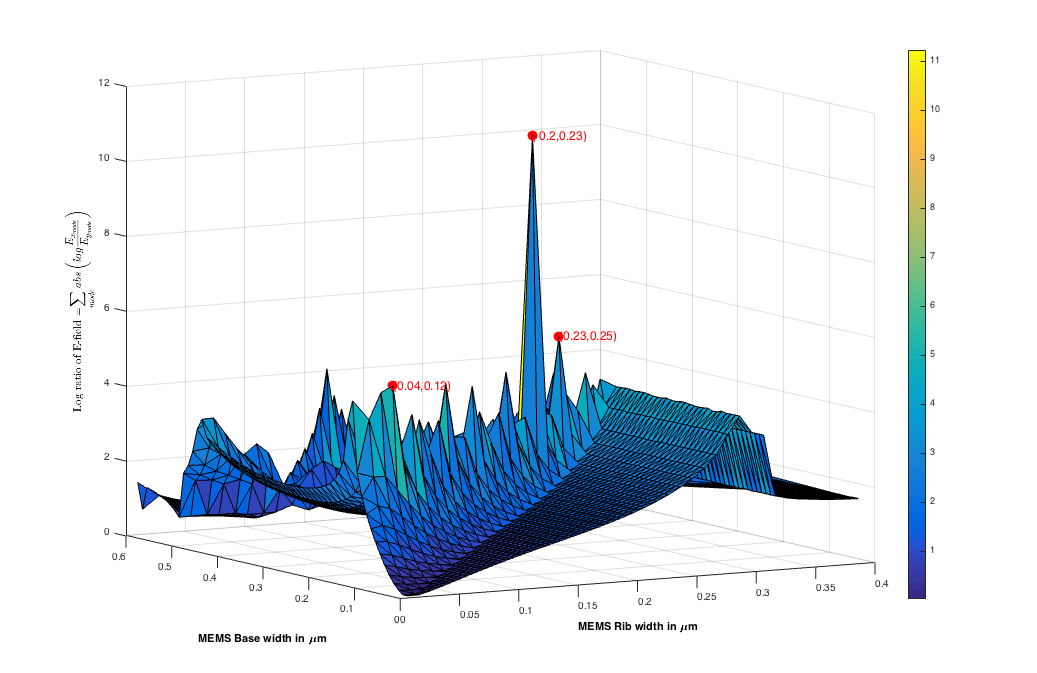
\includegraphics[width=1\textwidth]{3-graph-mode-sum-mems}
	\caption{Summation of real part of absolute value of the logarithmic ratio of $E_x$ and $E_y$ fields plotted against rib and total width in an area chart using MATLAB}
	\label{fig:3_graph_mode_sum_mems}
\end{figure}
		
\begin{figure}[H] %h
	\begin{subfigure}[t]{0.45\textwidth}
		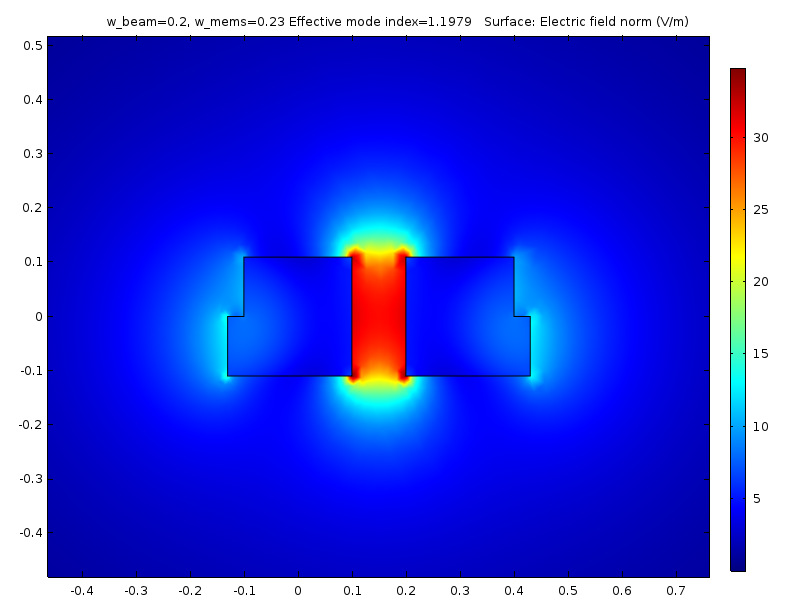
\includegraphics[width=\textwidth]{3-mems-mode1-200-230}
		\caption{\gls{te} mode with the \gls{mems} cross-section}
		\label{fig:3_mems_mode1_200_230}
	\end{subfigure}
	\hfill
	\begin{subfigure}[t]{0.45\textwidth}
		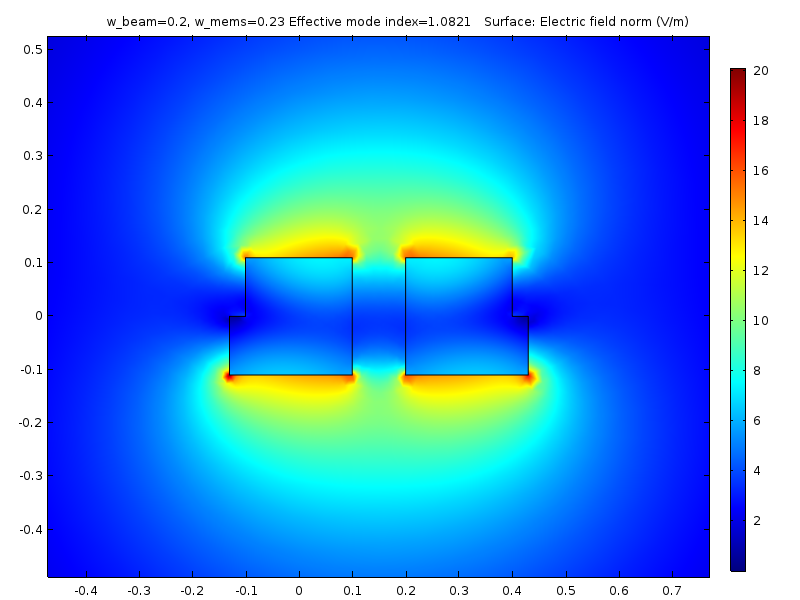
\includegraphics[width=\textwidth]{3-mems-mode2-200-230}
		\caption{\gls{tm} mode with the MEMS cross-section}
		\label{fig:3-mems-mode2-200-230}
	\end{subfigure}
	\caption{Modes in the cross-section with Rib width = 200nm, Slab width = 30nm, Slab height = Rib height = 110nm, in both bus and \gls{mems} waveguide, obtained using Comsol 2-D simulation}
\end{figure}

In this case the best dimensions for the \gls{mems} waveguide comes out as, $Rib_{width}$ = \SI{200}{nano meter}, $Rib_{height}$ = \SI{110}{nano meter}, $Base_{width}$ = \SI{230}{nano meter}, $Base_{height}$ = \SI{110}{nano meter}. Fig. \ref{fig:3-mems-mode2-200-230}, obtained using Comsol 2D simulation displays the port modes in the cross-section. This corroborates the claim that the \gls{mems} waveguide must be mirror image of the bus waveguide to inhibit \gls{pr}.

\subsubsection{Device tolerance}
When fabricating devices in nanometer scale often it is very difficult to control the device dimensions precisely. Hence, a brief study on simulation level is performed to check for deviance resulting due to variations in etch depth during the fabrication process discussed later in section \ref{sec:fab_process}.\\  

Since the wafer used in the fabrication process is of height 220nm, the different etch depths considered are 100nm and 130nm which corresponds to 120nm and 90nm slab height respectively. Fist 20 minimum values of $\sum _{mode}Real\left| \log _{10}\dfrac {E_{X_{mode}}} {E_{Y_{mode}}}\right|$, is plotted against $Rib_{width}$ and $Slab_{width}$ in the following figure in Fig. \ref{fig:3_graph_mode_sum_120nm_slab_height} for an etch depth of 100nm. 

\begin{figure}[H] %h
	\centering
	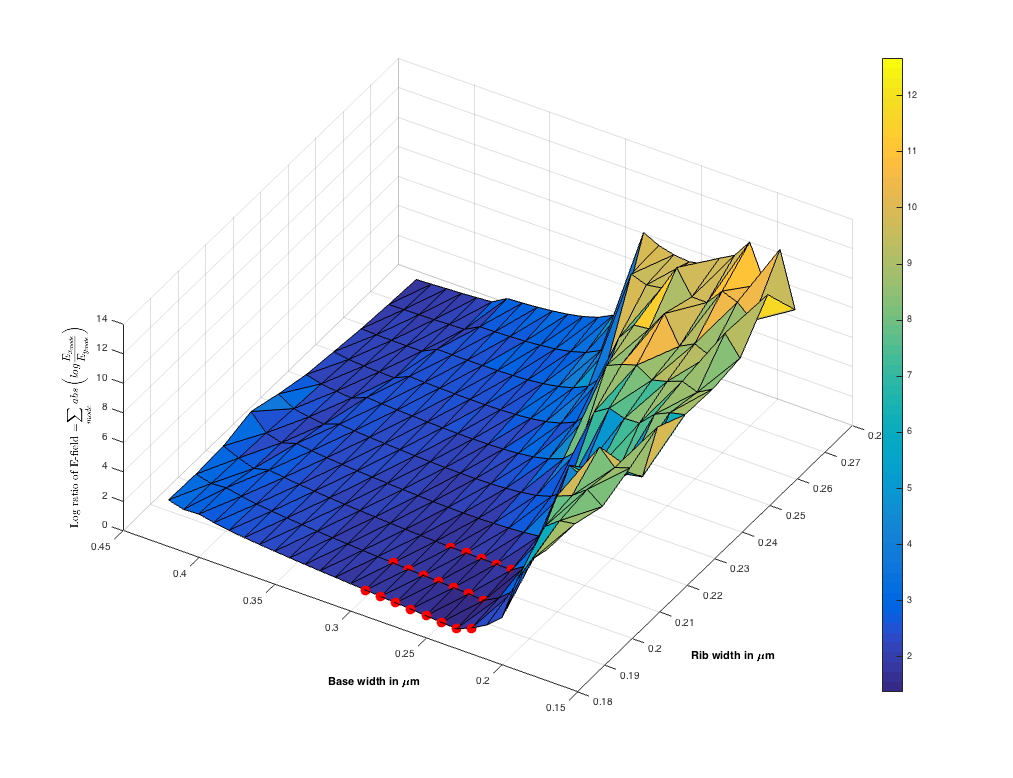
\includegraphics[width=1\textwidth]{3-graph-mode-sum-120nm-slab-height}
	\caption{20 least values, representing the summation of real part of absolute value of the logarithmic ratio of $E_x$ and $E_y$ fields, plotted against rib and total width in an area chart using MATLAB for Slab height = 120nm}
	\label{fig:3_graph_mode_sum_120nm_slab_height}
\end{figure}
\noindent It can be seen in the above Fig. \ref{fig:3_graph_mode_sum_120nm_slab_height} that the hybridized modes appear to be at $45^{\circ}$ around $230nm \leq Slab_{width} \leq 300nm$ and $180nm \leq Rib_{width} \leq 200nm$. So, if the $Rib_{width}$ and $Slab_{width}$ are controlled in the fabrication process, the device can still function in a modest way.\\

The same process is followed for a speculated etch depth of 130nm and the 20 best dimensions are plotted which comes out to be $230nm \leq Slab_{width} \leq 300nm$ and $160nm \leq Rib_{width} \leq 200nm$. The exact pairs can be identified in the Fig. \ref{fig:3_graph_mode_sum_90nm_slab_height}.
\begin{figure}[H] %h
	\centering
	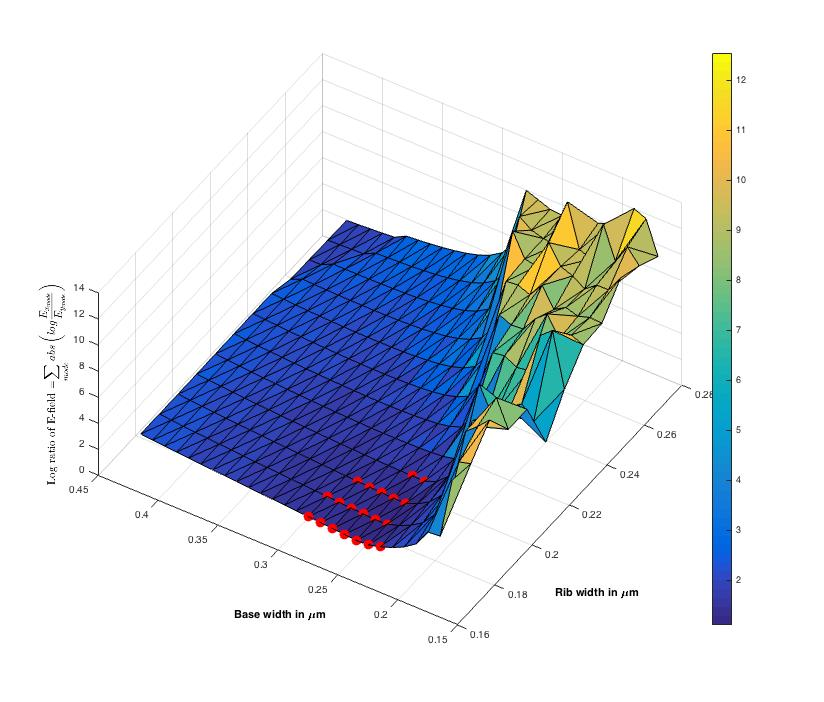
\includegraphics[width=1\textwidth]{3-graph-mode-sum-90nm-slab-height}
	\caption{20 least values, representing the summation of real part of absolute value of the logarithmic ratio of $E_x$ and $E_y$ fields, plotted against rib and total width in an area chart using MATLAB for Slab height = 90nm}
	\label{fig:3_graph_mode_sum_90nm_slab_height}
\end{figure}

\subsubsection{Representational design based on simulation}			

		\subsection{Design B: Tapered Si waveguide with horizontal gradual asymmetry on SOI with air cladding based on mode evolution}

\subsubsection{Optimized dimensions of bus waveguide}
		
\begin{figure}[H] %h
	\begin{subfigure}[t]{0.45\textwidth}
		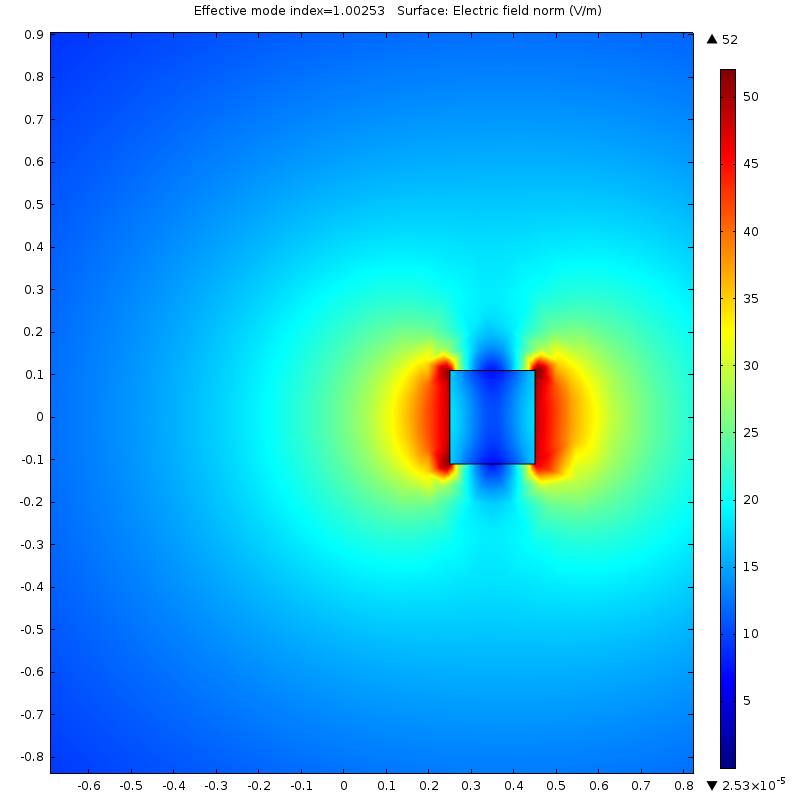
\includegraphics[width=\textwidth]{3-mode1-200-200}
		\caption{\gls{te} mode in the cross-section}
		\label{fig:3_mode1_200_200}
	\end{subfigure}
	\hfill
	\begin{subfigure}[t]{0.45\textwidth}
		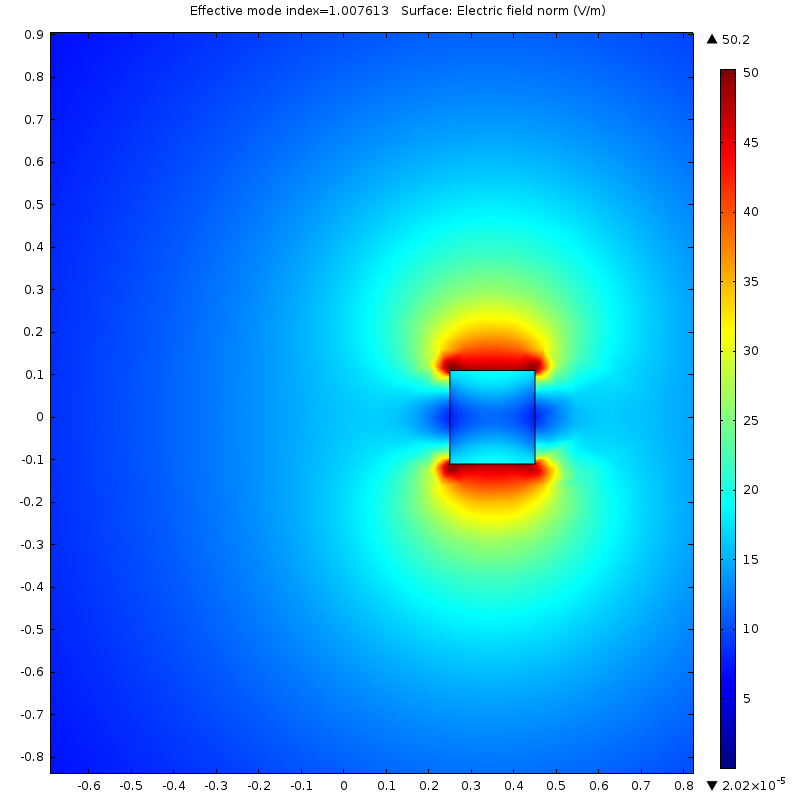
\includegraphics[width=\textwidth]{3-mode2-200-200}
		\caption{\gls{tm} mode in the cross-section}
		\label{fig:3_mode2_200_200}
	\end{subfigure}
	\caption{Hybrid modes in the cross-section with width = 200nm, height = 220nm, obtained using Comsol 2-D simulation}
\end{figure}

\subsubsection{Optimized dimensions of MEMS waveguide}	

\subsubsection{Device tolerance}

\subsubsection{Representational design based on simulation}

\end{document}
